\documentclass[12pt,openright,oneside,a4paper,brazil]{abntex2}

\usepackage{times}
\usepackage[T1]{fontenc}
\usepackage[utf8]{inputenc}
\usepackage{indentfirst}
\usepackage{hyperref}
\usepackage{color}
\usepackage{graphicx}
\usepackage{microtype}
\usepackage[ruled,vlined]{algorithm2e}
\usepackage{algorithmic}
\usepackage{float}
\usepackage{amsfonts,amsthm, amssymb, amsmath}
\usepackage{cancel}
\usepackage{verbatim}
\usepackage{multirow,multicol, array}
\usepackage{indentfirst}
\usepackage{subcaption}
\usepackage{xcolor, colortbl}
\usepackage{pdflscape}
\usepackage{lipsum}
\usepackage{syntax}
\usepackage{listings}
% \usepackage[brazilian,hyperpageref]{backref}
\usepackage[alf, abnt-emphasize=bf, bibjustif, recuo=0cm, abnt-etal-cite=2, abnt-etal-list=0]{abntex2cite}

\definecolor{blue}{RGB}{41,5,195}

\makeatletter
\hypersetup{
     	%pagebackref=true,
		pdftitle={\@title}, 
		pdfauthor={\@author},
    	pdfsubject={\imprimirpreambulo},
	    pdfcreator={Valdex Santos},
		pdfkeywords={abnt}{latex}{abntex}{abntex2}{relatório}, 
		colorlinks=true,
    	linkcolor=black,
    	citecolor=black,
    	filecolor=magenta,
		urlcolor=blue,
		bookmarksdepth=4
}

\titulo{COMPILADORES - TRABALHO FINAL}
\autor{	RAFAEL DIAS CAMPOS }
\local{Belo Horizonte-MG}
\data{2022}
\tipotrabalho{Relatório técnico sobre compiladores}
\preambulo{Relatório do compilador implementado no trabalho final da disciplina de Compiladores, ministrada pela professora Kecia Marques no primeiro semestre do ano letivo de 2022. }

\begin{document}
\frenchspacing 

\imprimircapa
\imprimirfolhaderosto*

\pdfbookmark[0]{\contentsname}{toc}
\tableofcontents*
\cleardoublepage

\setlength{\absparsep}{18pt}
\begin{resumo}
 Para este trabalho, foi definida pela professora a especificação de uma linguagem de programação. Em seguida, foi realizada a implementação de um compilador para esta linguagem.
 
 Este trabalho retrata o desenvolvimento e validação dos módulos do compilador: Analisador Léxico, Analisador Sintático, Analisador Semântico e Gerador de Código.
 
 \textbf{Palavras-chave}: Compilador, Léxico, Sintático, Semântico, Linguagem de Programação.
\end{resumo}

\textual

\chapter{Introdução}
\label{cap:intro}
Antes de se dar início a este trabalho, a professora Kecia Marques definiu a especificação de uma linguagem de programação para ser utilizada. A linguagem escolhida foi criada para este trabalho, e não retrata uma linguagem pré-existente.

A partir dessa especificação, foi primeiramente desenvolvido um Analisador Léxico para a linguagem, que é capaz de ler um arquivo fonte e emitir uma sequência de tokens.

Em seguida, foi desenvolvido um Analisador Sintático, que receberá os tokens provenientes do Analisador Léxico e irá produzir uma árvore de derivação para o arquivo fonte, com base na gramática definida para a linguagem.

Na próxima etapa, foi feita a criação de um Analisador Semântico, responsável por validar a árvore de derivação produzida pelo Analisador Sintático.

Finalmente, foi realizado um Gerador de Código, que recebe a árvore de derivação produzida pelo Analisador Sintático e validada pelo Analisador Semântico e produz seu código Assembly correspondente.

Além do processo de desenvolvimento dos módulos do compilador, esse trabalho também apresenta os resultados dos testes de validação realizados em cada etapa.

\section{Motivação}
\label{sec:motivacao}

Este trabalho foi realizado para colocar em prática os conhecimentos aprendidos em sala durante a disciplina de Compiladores.

Além disso, ele oferece uma introdução ao desenvolvimento de um Compilador para uma linguagem arbitrária e pode ser útil para o desenvolvimento de projetos similares no futuro.

\section{Objetivos}
\label{sec:objetivos}

O objetivo principal deste trabalho é produzir um compilador capaz de reconhecer a linguagem definida pela professora, e gerar o código correspondente.

Como objetivo secundário, foi escolhida a implementação de recuperação de erro, que possibilite a exibição de todos os erros presentes no código fonte com uma única execução do compilador.
\chapter{Utilização}
\label{cap:utilizacao}

\section{Download do Código}

O código desenvolvido para o compilador encontra-se no repositório do GitHub:

\href{https://github.com/RafaelDiasCampos/Compiler}{https://github.com/RafaelDiasCampos/Compiler}

\section{Compilação}

\subsection{Dependências}
Para realizar a compilação, primeiro é necessário instalar as seguintes dependências:

    \begin{lstlisting}
    g++
    cmake
    \end{lstlisting}

\subsection{Comando de Compilação}

Compile com o seguintes comandos:

    \begin{lstlisting}[language=bash]
    $ git clone https://github.com/RafaelDiasCampos/Compiler
    $ cd Compiler
    $ cmake .
    $ cmake --build .
    \end{lstlisting}

\section{Execução}

    \begin{lstlisting}[language=bash]
    $ ./Compiler file
    \end{lstlisting}
\chapter{Descrição da Linguagem}
\label{cap:descricaoLinguagem}

\section{Gramática}
\label{sec:gramatica}

A linguagem foi definida pela seguinte Gramática Livre de Contexto (em notação BNF):

\begin{grammar}

<program> ::= `routine' body

<body> ::= [<decl-list>] `begin' <stmt-list> `end'

<decl-list> ::= `declare' <decl> `;' {<decl> `;'}

<decl> ::= <type> <ident-list>

<ident-list> ::= <identifier> {`;' <identifier>}

<type> ::= `int` | `float' | `char'

<stmt-list> ::= <stmt> {`;' <stmt>}

<stmt> ::= <assign-stmt> | <if-stmt> | <while-stmt> | <repeat-stmt> | <read-stmt> | <write-stmt>

<assign-stmt> ::= <identifier> `:=' <simple-expr>

<if-stmt> ::= `if' <condition> `then' <stmt-list> `end'
              \alt `if' <condition> `then' <stmt-list> `else' <stmt-list> `end'
              
<condition> : <expression>

<repeat-stmt> ::= `repeat' <stmt-list> <stmt-suffix>

<stmt-suffix> ::= `until' <condition>

<while-stmt> ::= <stmt-prefix> <stmt-list> `end'

<stmt-prefix> ::= `while' <condition> `do'

<read-stmt> ::= `read' `(' <identifier> `)'

<write-stmt> ::= `write' `(` <writable> `)'

<writable> ::= <simple-expr> | <literal>

<expression> ::= <simple-expr> | <simple-expr> <relop> <simple-expr>

<simple-expr> ::= <term> | <simple-expr> <addop> <term>

<term> ::= <factor-a> | <term> <mulop> <factor-a>

<factor-a> ::= <factor> | `not' <factor> | `-' <factor>

<factor> ::= <identifier> | <constant> | `(' <expression> `)'

<relop> ::= `=' | `>' | `>=' | `<' | `<=' | `<>'

<addop> ::= `+' | `-' | `or'

<mulop> ::= `*' | `/' | `and'

<constant> ::= <integer_const> | <float_const> | <char_const>

\end{grammar}

\section{Tokens}
\label{sec:tokens}

Os tokens foram definidos a partir das seguintes expressões regulares:

\begin{grammar}

<integer_const> ::= <digit>+

<float_const> ::= <digit>+ `.' <digit>+

<char_const> ::= `\'' <carac> `\''

<literal> ::= `\"' <caractere>* `\"'

<identifier> ::= <letter> (<letter> | <digit>)*

<letter> ::= [A-za-z]

<digit> ::= [0-9]

<carac> ::= .*

\end{grammar}

\section{Outras características}
\label{sec:caracteristicas}

A linguagem apresenta algumas outras características, descritas a seguir:

\begin{itemize}
\item Palavras-chave são reservadas
\item Variáveis devem ser declaradas antes de seu uso
\item Comentários se iniciam por '\%' e terminal com '\%'
\item Valores do tipo inteiro podem ser atribuídos a variáveis do tipo float, mas o inverso não é permitido
\item O resultado de uma divisão é sempre um float
\item A linguagem é case-sensitive
\end{itemize}
\chapter{Analisador Léxico}
\label{cap:lexico}
Neste capítulo será descrita a implementação do Analisador Léxico. Esse componente do compilador é responsável por ler o arquivo fonte e transformá-lo em uma sequência de tokens.

\section{Definição dos Tokens}
\label{sec:lexicoDefinicaoTokens}
Inicialmente, foi necessário definir quais serão os tokens da linguagem nessa implementação. Com base, na gramática apresentada na seção \ref{sec:gramatica}, foi definida a seguinte lista de tokens:

Tokens Básicos: ROUTINE, BEGIN, END, DECLARE, INT, FLOAT, CHAR, IF, THEN, ELSE, REPEAT, UNTIL, WHILE, DO, READ, WRITE, NOT, OR, AND, ASSIGN, ADD, SUB, MUL, DIV, COMP\_EQ, COMP\_NE, COMP\_GT, COMP\_GE, COMP\_LT, COMP\_LE, OPEN\_BRACES, CLOSE\_BRACES, SEMICOLON, COMMA

Constantes: CONST\_INT, CONST\_FLOAT, CONST\_CHAR, CONST\_STRING

Identificadores: ID

Outros Tokens: END\_OF\_FILE, INVALID\_TOKEN, ERROR

\section{Estrutura do programa}
\label{sec:lexicoEstrutura}
Foi criada uma classe Token para representar os tokens da linguagem.
Essa classe possui um enum TokenType utilizado para armazenar o tipo de token que o objeto representa, com base na lista apresentada na seção \ref{sec:lexicoDefinicaoTokens}.
Para representar constantes, foi definida uma classe derivada de Token, chamada de ValueType.
Dessa classe foram derivadas as classes TokenConstInt, TokenConstFloat, TokenConstChar e TokenConstString, com cada objeto armazenando seu respectivo valor.
Finalmente, para Identificadores, foi criada a classe TokenId, derivada de Token, que armazena seu id e uma referência para o ValueType com seu respectivo valor.

Para navegar no arquivo fonte, foi criada uma classe FileHandler, que é responsável por abrir e ler o arquivo.
Essa classe também armazena um objeto do tipo struct chamado FilePosition, que indica a linha e a coluna atual do arquivo e também oferece uma função putback que retorna o último caractere lido para o buffer.

A implementação da tabela de símbolos foi realizada por meio da classe SymbolTable.
Ela armazena um unordered\_map (correspondente a um hash map) que relaciona o nome de um símbolo com seu respectivo objeto do tipo Token.
Ela implementa dois métodos, insertSymbol() e insertId(), que podem ser utilizados para inserir um novo token na tabela, ou para retornar o token já existente.

O Analisador Léxico em si foi implementado por meio de um parser recursivo descendente. Ele possui um método principal, getNextToken(), que retorna um ponteiro para o próximo Token lido.
Para evitar criar tokens de forma desnecessária, ele armazena um array com os tokens básicos, já que eles são imutáveis.
Ele também armazena um vetor com os ValueTokens que são criados.
Essa parte é necessária pois eles são alocados de forma dinâmica na memória e portanto é preciso armazenar uma referência para posteriormente liberar a memória, e, no caso dos ValueTypes, não se pode saber a tempo de compilação até em que momento eles serão utilizados.
O Analisador Léxico também armazena o FileHandler e a SymbolTable, para seu uso.
Ao se iniciar a execução, a tabela de símbolos é populada com as palavras reservadas da linguagem, pois dessa forma elas podem ser tratadas pelo Léxico como identificadores durante o processo de parsing do arquivo.

A seguir encontra-se o diagrama de classes do programa, no estilo UML:

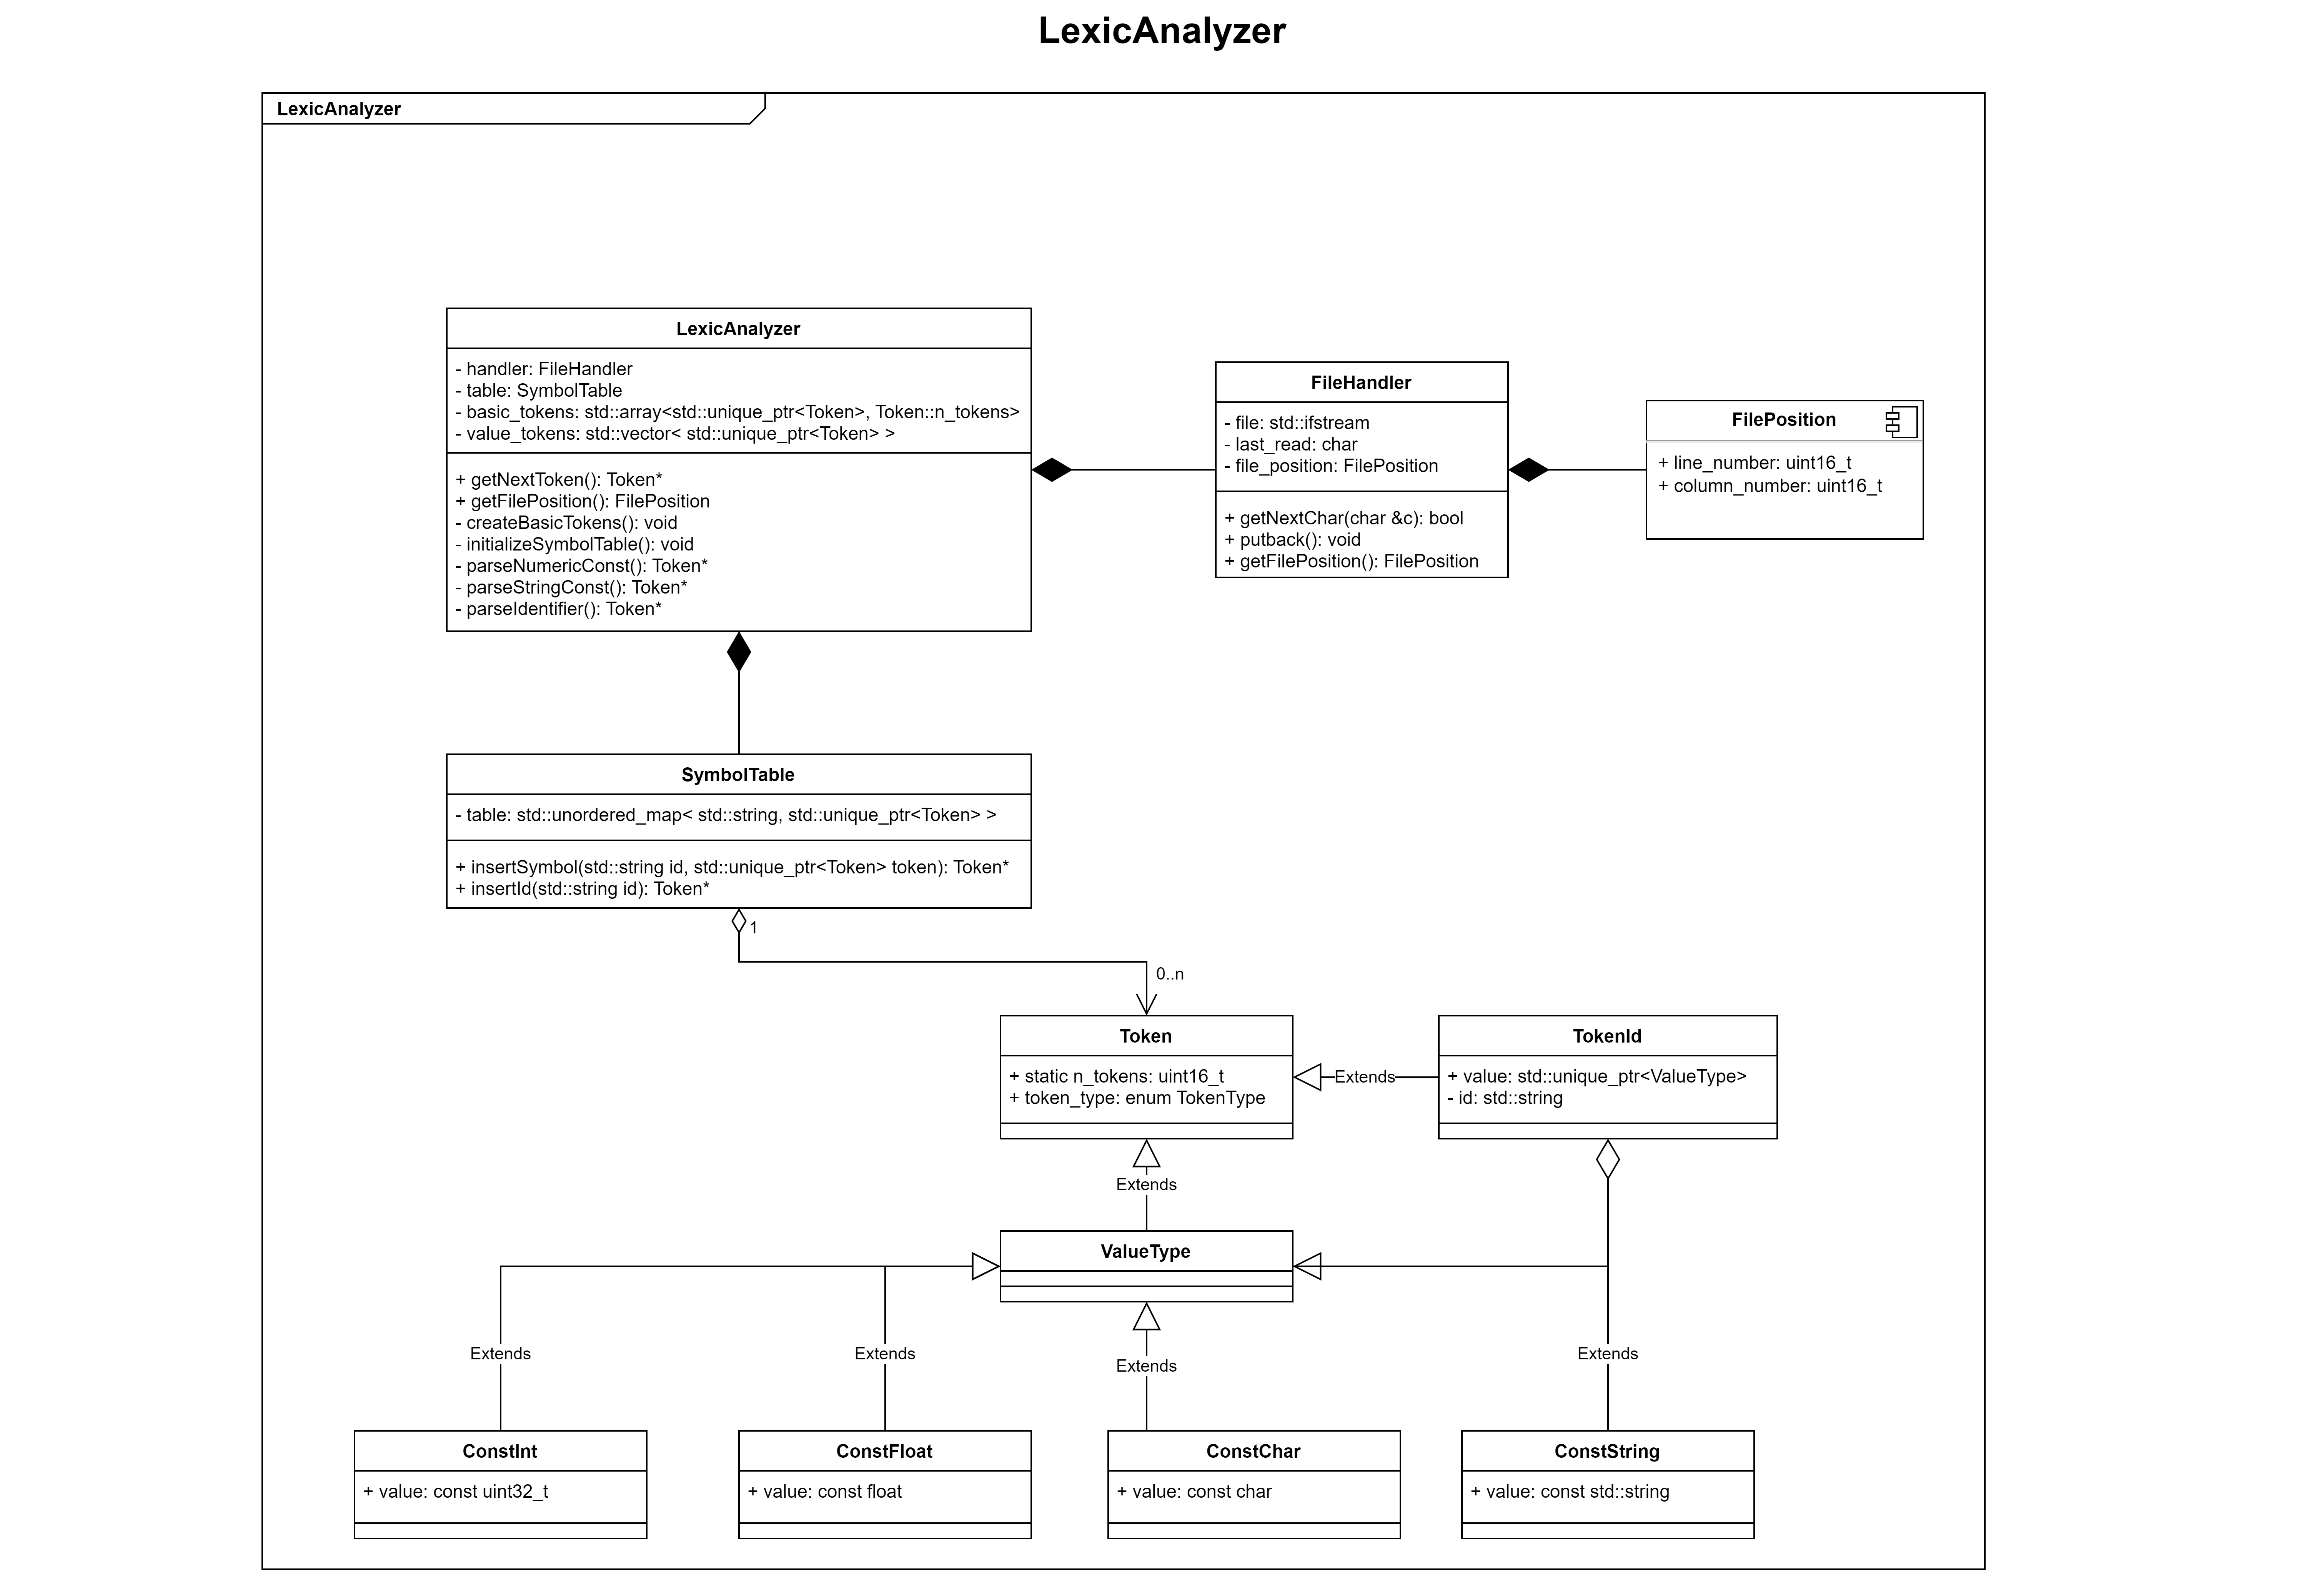
\includegraphics[width=\linewidth]{2-Imagens/Lexico-UML.png}

\section{Testes de validação}
\label{sec:lexicoTestes}

\subsection{Teste 01}
\label{subsec:lexicoTeste01}

\subsubsection{Código Original}
\verbatiminput{../tests/1/original.txt}

Saida do Compilador:

\verbatiminput{3-testes/lexico/1/original.txt}

\subsection{Teste 02}
\label{subsec:lexicoTeste02}

\subsubsection{Código Original}
\verbatiminput{../tests/2/original.txt}

Saida do Compilador:


\verbatiminput{3-testes/lexico/2/original.txt}

\subsubsection{Código com Comentário Corrigido}
\verbatiminput{../tests/2/fixedComment.txt}

Saida do Compilador:


\verbatiminput{3-testes/lexico/2/fixedComment.txt}

\subsubsection{Código Corrigido}
\verbatiminput{../tests/2/fixedLexic.txt}

Saida do Compilador:


\verbatiminput{3-testes/lexico/2/fixedLexic.txt}

\subsection{Teste 03}
\label{subsec:lexicoTeste03}

\subsubsection{Código Original}
\verbatiminput{../tests/3/original.txt}

Saida do Compilador:


\verbatiminput{3-testes/lexico/3/original.txt}
\subsection{Teste 04}
\label{subsec:lexicoTeste04}

\subsubsection{Código Original}
\verbatiminput{../tests/4/original.txt}

Saida do Compilador:


\verbatiminput{3-testes/lexico/4/original.txt}

\subsubsection{Código com String Corrigida}
\verbatiminput{../tests/4/fixedString.txt}

Saida do Compilador:


\verbatiminput{3-testes/lexico/4/fixedString.txt}

\subsubsection{Código Corrigido}
\verbatiminput{../tests/4/fixedLexic.txt}

Saida do Compilador:


\verbatiminput{3-testes/lexico/4/fixedLexic.txt}

\subsection{Teste 05}
\label{subsec:lexicoTeste05}

\subsubsection{Código Original}
\verbatiminput{../tests/5/original.txt}

Saida do Compilador:


\verbatiminput{3-testes/lexico/5/original.txt}

\subsubsection{Código com String Corrigida}
\verbatiminput{../tests/5/fixedString.txt}

Saida do Compilador:


\verbatiminput{3-testes/lexico/5/fixedString.txt}

\subsubsection{Código Corrigido}
\verbatiminput{../tests/5/fixedLexic.txt}

Saida do Compilador:


\verbatiminput{3-testes/lexico/5/fixedLexic.txt}

\subsection{Teste 06}
\label{subsec:lexicoTeste06}

\subsubsection{Código Original}
\verbatiminput{../tests/6/original.txt}

Saida do Compilador:


\verbatiminput{3-testes/lexico/6/original.txt}

\subsubsection{Código Corrigido}
\verbatiminput{../tests/6/fixedLexic.txt}

Saida do Compilador:


\verbatiminput{3-testes/lexico/6/fixedLexic.txt}

\subsection{Teste 07}
\label{subsec:lexicoTeste07}

\subsubsection{Código Original}
\verbatiminput{../tests/7/original.txt}

Saida do Compilador:


\verbatiminput{3-testes/lexico/7/original.txt}

\subsubsection{Código Corrigido}
\verbatiminput{../tests/7/fixedLexic.txt}

Saida do Compilador:


\verbatiminput{3-testes/lexico/7/fixedLexic.txt}
\chapter{Analisador Sintático}
\label{cap:sintatico}

\section{Alteração na Gramática}
\label{sec:sintaticoAlteracaoGramatica}
A gramática original apresenta recursão a esquerda, o que impossibilita a construção de um parser recursivo descendente que a reconheça.
Por isso, foi feita a seguinte modificação na gramática para eliminar essa recursão:

\begin{grammar}
    
    <program> ::= `routine' body
    
    <body> ::= [<decl-list>] `begin' <stmt-list> `end'
    
    <decl-list> ::= `declare' <decl> `;' {<decl> `;'}
    
    <decl> ::= <type> <ident-list>
    
    <ident-list> ::= <identifier> {`;' <identifier>}
    
    <type> ::= `int` | `float' | `char'
    
    <stmt-list> ::= <stmt> {`;' <stmt>}
    
    <stmt> ::= <assign-stmt> | <if-stmt> | <while-stmt> | <repeat-stmt> | <read-stmt> | <write-stmt>
    
    <assign-stmt> ::= <identifier> `:=' <simple-expr-a>
    
    <if-stmt> ::= `if' <condition> `then' <stmt-list> `end'
                  \alt `if' <condition> `then' <stmt-list> `else' <stmt-list> `end'
                  
    <condition> : <expression>
    
    <repeat-stmt> ::= `repeat' <stmt-list> <stmt-suffix>
    
    <stmt-suffix> ::= `until' <condition>
    
    <while-stmt> ::= <stmt-prefix> <stmt-list> `end'
    
    <stmt-prefix> ::= `while' <condition> `do'
    
    <read-stmt> ::= `read' `(' <identifier> `)'
    
    <write-stmt> ::= `write` `(` <writable> `)'
    
    <writable> ::= <simple-expr-a> | <literal>
    
    <expression> ::= <simple-expr-a> | <simple-expr-a> <relop> <simple-expr-a>
    
    <simple-expr-a> ::= <term-a> <simple-expr>

    <simple-expr> ::= <addop> <term-a> <simple-expr> | lambda
    
    <term-a> ::= <factor-a> <term>

    <term> ::= <mulop> <factor-a> <term> | lambda
    
    <factor-a> ::= <factor> | `not' <factor> | `-' <factor>
    
    <factor> ::= <identifier> | <constant> | `(' <expression> `)'
    
    <relop> ::= `=' | `>' | `>=' | `<' | `<=' | `<>'
    
    <addop> ::= `+' | `-' | `or'
    
    <mulop> ::= `*' | `/' | `and'
    
    <constant> ::= <integer_const> | <float_const> | <char_const>
    
    \end{grammar}

\section{Calculo de First e Follow}
\label{sec:sintaticoFirstFollow}

Para ajudar na implementação do compilador, foi realizad o cálculo do First e Follow para cada não-terminal da gramática:

    \begin{itemize}
        \item \textbf{First}:
        \begin{itemize}
            \item \textit{<program>}: `routine'
            \item \textit{<body>}: `begin' | `declare'
            \item \textit{<decl-list>}: `declare'
            \item \textit{<decl>}: `int' | `float' | `char'
            \item \textit{<ident-list>}: <identifier>
            \item \textit{<type>}: `int' | `float' | `char'
            \item \textit{<stmt-list>}: <identifier> | `if' | `while' | `repeat' | `read' | `write'
            \item \textit{<stmt>}: <identifier> | `if' | `while' | `repeat' | `read' | `write'
            \item \textit{<assign-stmt>}: <identifier>
            \item \textit{<if-stmt>}: `if'
            \item \textit{<condition>}: <identifier> | `(' | `not' | `-' | <integer_const> | <float_const> | <char_const>
            \item \textit{<repeat-stmt>}: `repeat'
            \item \textit{<stmt-suffix>}: `until'
            \item \textit{<while-stmt>}: `while'
            \item \textit{<stmt-prefix>}: `while'
            \item \textit{<read-stmt>}: `read'
            \item \textit{<write-stmt>}: `write'
            \item \textit{<writable>}: <identifier> | `(' | `not' | `-' | <literal> | <integer_const> | <float_const> | <char_const>
            \item \textit{<expression>}: <identifier> | `(' | `not' | `-' | <integer_const> | <float_const> | <char_const>
            \item \textit{<simple-expr-a>}: <identifier> | `(' | `not' | `-' | <integer_const> | <float_const> | <char_const>
            \item \textit{<simple-expr>}: `-' | `+' | `or' | lambda
            \item \textit{<term-a>}: <identifier> | `(' | `not' | `-' | <integer_const> | <float_const> | <char_const>
            \item \textit{<term>}: `*' | `/' | `and' | lambda
            \item \textit{<factor-a>}: <identifier> | `(' | `not' | `-' | <integer_const> | <float_const> | <char_const>
            \item \textit{<factor>}: <identifier> | `(' | <integer_const> | <float_const> | <char_const>
            \item \textit{<relop>}: `=' | `>' | `>=' | `<' | `<=' | `<>'
            \item \textit{<addop>}: `+' | `-' | `or'
            \item \textit{<mulop>}: `*' | `/' | `and'
            \item \textit{<constant>}: <integer_const> | <float_const> | <char_const>
        \end{itemize}
        \item \textbf{Follow}:
        \begin{itemize}
            \item \textit{<program>}: \$
            \item \textit{<body>}: \$
            \item \textit{<decl-list>}: `begin'
            \item \textit{<decl>}: `;'
            \item \textit{<ident-list>}: `;'
            \item \textit{<type>}: <identifier> 
            \item \textit{<stmt-list>}: `end' | `else' | `until'
            \item \textit{<stmt>}: `end' | `else' | `until'
            \item \textit{<assign-stmt>}: `end' | `else' | `until'
            \item \textit{<if-stmt>}: `end' | `else' | `until'
            \item \textit{<condition>}: `end' | `else' | `until' | `then' | `do'
            \item \textit{<repeat-stmt>}: `end' | `else' | `until'
            \item \textit{<stmt-suffix>}: `end' | `else' | `until'
            \item \textit{<while-stmt>}: `end' | `else' | `until'
            \item \textit{<stmt-prefix>}: <identifier> | `if' | `repeat' | `while' | `read' | `write'
            \item \textit{<read-stmt>}: `end' | `else' | `until' 
            \item \textit{<write-stmt>}: `end' | `else' | `until' 
            \item \textit{<writable>}: `)'
            \item \textit{<expression>}: `end' | `then' | `else' | `until' | `do' | `)'
            \item \textit{<simple-expr-a>}: `end' | `then' | `else' | `until' | `do' | `)' | `=' | `>' | `>=' | `<' | `<=' | `<>'
            \item \textit{<simple-expr>}: `end' | `then' | `else' | `until' | `do' | `)' | `=' | `>' | `>=' | `<' | `<=' | `<>'
            \item \textit{<term-a>}: `end' | `then' | `else' | `until' | `do' | `)' | `-' | `+' | `or' | `=' | `>' | `>=' | `<' | `<=' | `<>'
            \item \textit{<term>}: `end' | `then' | `else' | `until' | `do' | `)' | `-' | `+' | `or' | `=' | `>' | `>=' | `<' | `<=' | `<>'
            \item \textit{<factor-a>}: `end' | `then' | `else' | `until' | `do' | `)' | `-' | `+' | `or' | `=' | `>' | `>=' | `<' | `<=' | `<>' | `*' | `/' | `and'
            \item \textit{<factor>}: `end' | `then' | `else' | `until' | `do' | `)' | `-' | `+' | `or' | `=' | `>' | `>=' | `<' | `<=' | `<>' | `*' | `/' | `and'
            \item \textit{<relop>}: <identifier> | `(' | `not' | `-' | <integer_const> | <float_const> | <char_const>
            \item \textit{<addop>}: <identifier> | `(' | `not' | `-' | <integer_const> | <float_const> | <char_const>
            \item \textit{<mulop>}: <identifier> | `(' | `not' | `-' | <integer_const> | <float_const> | <char_const>
            \item \textit{<constant>}: `end' | `then' | `else' | `until' | `do' | `)' | `-' | `+' | `or' | `=' | `>' | `>=' | `<' | `<=' | `<>' | `*' | `/' | `and'
        \end{itemize}
    \end{itemize}
    
\section{Estrutura do Programa}
\label{sec:sintaticoEstrutura}
Foi feita implementação de um Parser Recursivo Descendente para reconhecer a gramática da linguagem tilizando o algoritmo de parsing LL(1) .

Cada regra da gramática foi representada por uma classe que herda de \textbf{Construct}.
Essas regras recebem como parâmetros objetos do tipo \textbf{Token} ou do tipo \textbf{Construct} que representam a derivação escolhida para essa regra. 

\section{Recuperação de Erros}
Para recuperar os erros de sintaxe, foi utilizado o método baseado na análise do Follow de cada regra da gramática.
Ao encontrar um erro na construção de uma regra, o programa "come"  novos Tokens até encontrar um que pertence ao Follow da regra que estava sendo construída.
Dessa forma, é garantido que pelo menos o início da construção da regra seguinte será possível, o que permite um reconhecimento maior de erros.


\section{Testes de validação}
\label{sec:sintaticoTestes}

\subsection{Teste 01}
\label{subsec:sintaticoTeste01}

\subsubsection{Código Original}
\verbatiminput{../tests/1/original.txt}

Saida do Compilador:

\verbatiminput{3-testes/sintatico/1/original.txt}

\subsubsection{Código Corrigido}
\verbatiminput{../tests/1/fixedSyntatic.txt}

Saida do Compilador:

\verbatiminput{3-testes/sintatico/1/fixedSyntatic.txt}

\subsection{Teste 02}
\label{subsec:sintaticoTeste02}

\subsubsection{Código Original}
\verbatiminput{../tests/2/fixedLexic.txt}

Saida do Compilador:


\verbatiminput{3-testes/sintatico/2/fixedLexic.txt}

\subsubsection{Código Corrigido}
\verbatiminput{../tests/2/fixedSyntatic.txt}

Saida do Compilador:


\verbatiminput{3-testes/sintatico/2/fixedSyntatic.txt}

\subsection{Teste 03}
\label{subsec:sintaticoTeste03}

\subsubsection{Código Original}
\verbatiminput{../tests/3/original.txt}

Saida do Compilador:


\verbatiminput{3-testes/sintatico/3/original.txt}

\subsection{Teste 04}
\label{subsec:sintaticoTeste04}

\subsubsection{Código Original}
\verbatiminput{../tests/4/fixedLexic.txt}

Saida do Compilador:


\verbatiminput{3-testes/sintatico/4/fixedLexic.txt}

\subsubsection{Código Corrigido}
\verbatiminput{../tests/4/fixedSyntatic.txt}

Saida do Compilador:


\verbatiminput{3-testes/sintatico/4/fixedSyntatic.txt}

\subsection{Teste 05}
\label{subsec:sintaticoTeste05}

\subsubsection{Código Original}
\verbatiminput{../tests/5/fixedLexic.txt}

Saida do Compilador:


\verbatiminput{3-testes/sintatico/5/fixedLexic.txt}

\subsubsection{Código com Token Routine}
\verbatiminput{../tests/5/fixedRoutine.txt}

Saida do Compilador:


\verbatiminput{3-testes/sintatico/5/fixedRoutine.txt}


\subsubsection{Código Corrigido}
\verbatiminput{../tests/5/fixedSyntatic.txt}

Saida do Compilador:


\verbatiminput{3-testes/sintatico/5/fixedSyntatic.txt}

\subsection{Teste 06}
\label{subsec:sintaticoTeste06}

\subsubsection{Código Original}
\verbatiminput{../tests/6/fixedLexic.txt}

Saida do Compilador:


\verbatiminput{3-testes/sintatico/6/fixedLexic.txt}

\subsubsection{Código Corrigido}
\verbatiminput{../tests/6/fixedSyntatic.txt}

Saida do Compilador:


\verbatiminput{3-testes/sintatico/6/fixedSyntatic.txt}

\subsection{Teste 07}
\label{subsec:sintaticoTeste07}

\subsubsection{Código Original}
\verbatiminput{../tests/7/fixedLexic.txt}

Saida do Compilador:


\verbatiminput{3-testes/sintatico/7/fixedLexic.txt}

\subsubsection{Código Corrigido}
\verbatiminput{../tests/7/fixedSyntatic.txt}

Saida do Compilador:


\verbatiminput{3-testes/sintatico/7/fixedSyntatic.txt}
\chapter{Analisador Semântico}
\label{cap:semantico}
\chapter{Gerador de Código}
\label{cap:geradorCodigo}
\chapter{Conclusões}
\label{cap:conclusoes}

\end{document}